\documentclass[1p]{elsarticle_modified}
%\bibliographystyle{elsarticle-num}

%\usepackage[colorlinks]{hyperref}
%\usepackage{abbrmath_seonhwa} %\Abb, \Ascr, \Acal ,\Abf, \Afrak
\usepackage{amsfonts}
\usepackage{amssymb}
\usepackage{amsmath}
\usepackage{amsthm}
\usepackage{scalefnt}
\usepackage{amsbsy}
\usepackage{kotex}
\usepackage{caption}
\usepackage{subfig}
\usepackage{color}
\usepackage{graphicx}
\usepackage{xcolor} %% white, black, red, green, blue, cyan, magenta, yellow
\usepackage{float}
\usepackage{setspace}
\usepackage{hyperref}

\usepackage{tikz}
\usetikzlibrary{arrows}

\usepackage{multirow}
\usepackage{array} % fixed length table
\usepackage{hhline}

%%%%%%%%%%%%%%%%%%%%%
\makeatletter
\renewcommand*\env@matrix[1][\arraystretch]{%
	\edef\arraystretch{#1}%
	\hskip -\arraycolsep
	\let\@ifnextchar\new@ifnextchar
	\array{*\c@MaxMatrixCols c}}
\makeatother %https://tex.stackexchange.com/questions/14071/how-can-i-increase-the-line-spacing-in-a-matrix
%%%%%%%%%%%%%%%

\usepackage[normalem]{ulem}

\newcommand{\msout}[1]{\ifmmode\text{\sout{\ensuremath{#1}}}\else\sout{#1}\fi}
%SOURCE: \msout is \stkout macro in https://tex.stackexchange.com/questions/20609/strikeout-in-math-mode

\newcommand{\cancel}[1]{
	\ifmmode
	{\color{red}\msout{#1}}
	\else
	{\color{red}\sout{#1}}
	\fi
}

\newcommand{\add}[1]{
	{\color{blue}\uwave{#1}}
}

\newcommand{\replace}[2]{
	\ifmmode
	{\color{red}\msout{#1}}{\color{blue}\uwave{#2}}
	\else
	{\color{red}\sout{#1}}{\color{blue}\uwave{#2}}
	\fi
}

\newcommand{\Sol}{\mathcal{S}} %segment
\newcommand{\D}{D} %diagram
\newcommand{\A}{\mathcal{A}} %arc


%%%%%%%%%%%%%%%%%%%%%%%%%%%%%5 test

\def\sl{\operatorname{\textup{SL}}(2,\Cbb)}
\def\psl{\operatorname{\textup{PSL}}(2,\Cbb)}
\def\quan{\mkern 1mu \triangleright \mkern 1mu}

\theoremstyle{definition}
\newtheorem{thm}{Theorem}[section]
\newtheorem{prop}[thm]{Proposition}
\newtheorem{lem}[thm]{Lemma}
\newtheorem{ques}[thm]{Question}
\newtheorem{cor}[thm]{Corollary}
\newtheorem{defn}[thm]{Definition}
\newtheorem{exam}[thm]{Example}
\newtheorem{rmk}[thm]{Remark}
\newtheorem{alg}[thm]{Algorithm}

\newcommand{\I}{\sqrt{-1}}
\begin{document}

%\begin{frontmatter}
%
%\title{Boundary parabolic representations of knots up to 8 crossings}
%
%%% Group authors per affiliation:
%\author{Yunhi Cho} 
%\address{Department of Mathematics, University of Seoul, Seoul, Korea}
%\ead{yhcho@uos.ac.kr}
%
%
%\author{Seonhwa Kim} %\fnref{s_kim}}
%\address{Center for Geometry and Physics, Institute for Basic Science, Pohang, 37673, Korea}
%\ead{ryeona17@ibs.re.kr}
%
%\author{Hyuk Kim}
%\address{Department of Mathematical Sciences, Seoul National University, Seoul 08826, Korea}
%\ead{hyukkim@snu.ac.kr}
%
%\author{Seokbeom Yoon}
%\address{Department of Mathematical Sciences, Seoul National University, Seoul, 08826,  Korea}
%\ead{sbyoon15@snu.ac.kr}
%
%\begin{abstract}
%We find all boundary parabolic representation of knots up to 8 crossings.
%
%\end{abstract}
%\begin{keyword}
%    \MSC[2010] 57M25 
%\end{keyword}
%
%\end{frontmatter}

%\linenumbers
%\tableofcontents
%
\newcommand\colored[1]{\textcolor{white}{\rule[-0.35ex]{0.8em}{1.4ex}}\kern-0.8em\color{red} #1}%
%\newcommand\colored[1]{\textcolor{white}{ #1}\kern-2.17ex	\textcolor{white}{ #1}\kern-1.81ex	\textcolor{white}{ #1}\kern-2.15ex\color{red}#1	}

{\Large $\underline{11n_{178}~(K11n_{178})}$}

\setlength{\tabcolsep}{10pt}
\renewcommand{\arraystretch}{1.6}
\vspace{1cm}\begin{tabular}{m{100pt}>{\centering\arraybackslash}m{274pt}}
\multirow{5}{120pt}{
	\centering
	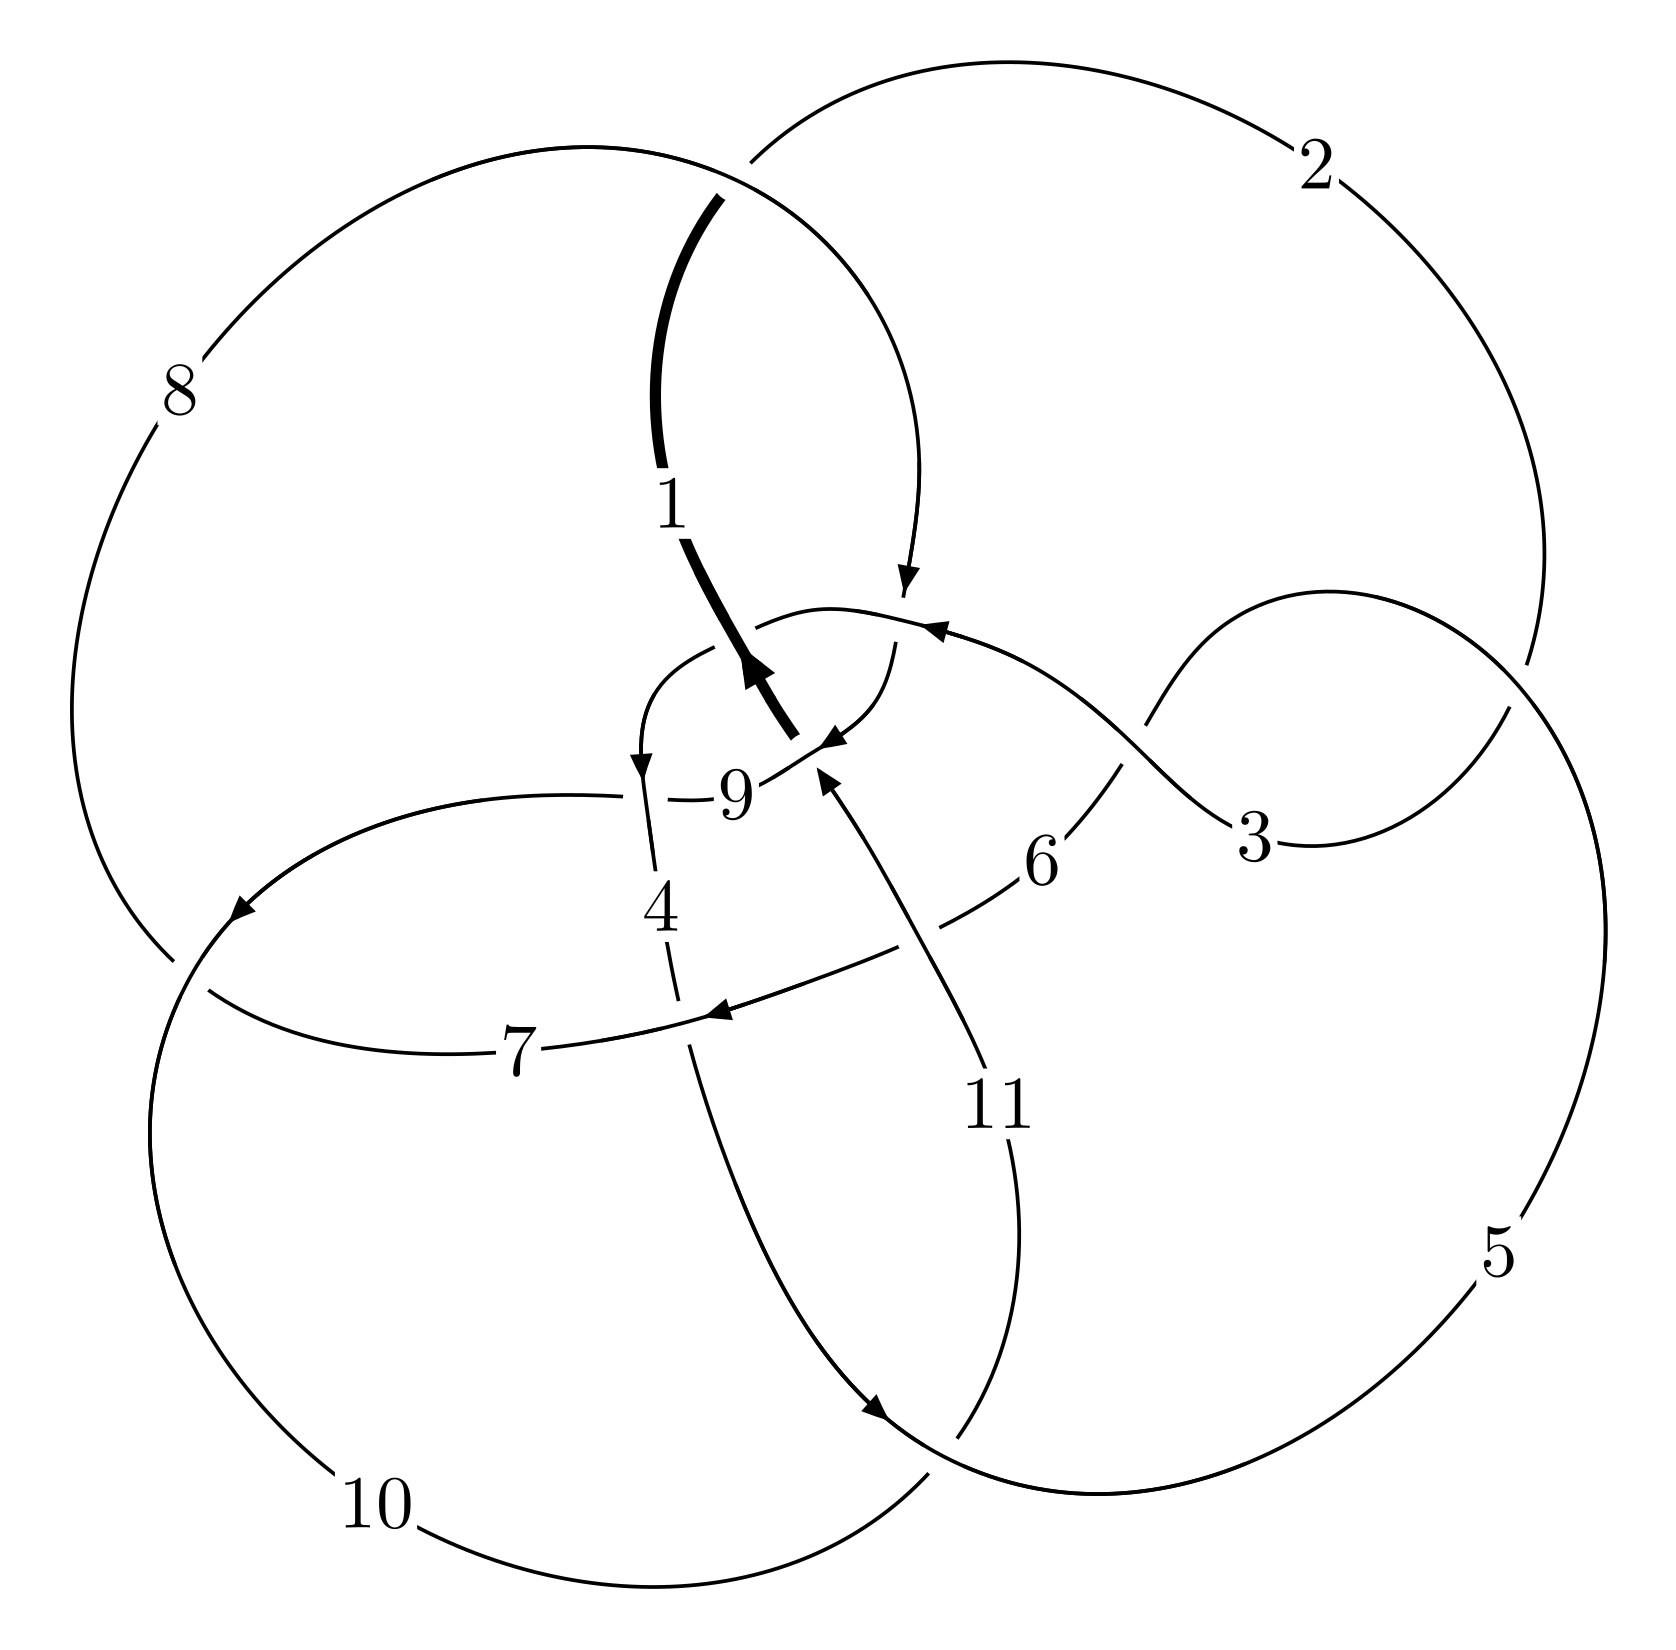
\includegraphics[width=112pt]{../../../GIT/diagram.site/Diagrams/png/794_11n_178.png}\\
\ \ \ A knot diagram\footnotemark}&
\allowdisplaybreaks
\textbf{Linearized knot diagam} \\
\cline{2-2}
 &
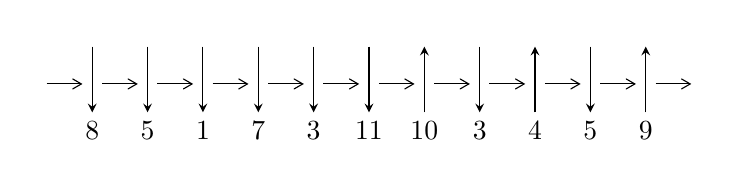
\begin{tikzpicture}[x=20pt, y=17pt]
	% nodes
	\node (C0) at (0, 0) {};
	\node (C1) at (1, 0) {};
	\node (C1U) at (1, +1) {};
	\node (C1D) at (1, -1) {8};

	\node (C2) at (2, 0) {};
	\node (C2U) at (2, +1) {};
	\node (C2D) at (2, -1) {5};

	\node (C3) at (3, 0) {};
	\node (C3U) at (3, +1) {};
	\node (C3D) at (3, -1) {1};

	\node (C4) at (4, 0) {};
	\node (C4U) at (4, +1) {};
	\node (C4D) at (4, -1) {7};

	\node (C5) at (5, 0) {};
	\node (C5U) at (5, +1) {};
	\node (C5D) at (5, -1) {3};

	\node (C6) at (6, 0) {};
	\node (C6U) at (6, +1) {};
	\node (C6D) at (6, -1) {11};

	\node (C7) at (7, 0) {};
	\node (C7U) at (7, +1) {};
	\node (C7D) at (7, -1) {10};

	\node (C8) at (8, 0) {};
	\node (C8U) at (8, +1) {};
	\node (C8D) at (8, -1) {3};

	\node (C9) at (9, 0) {};
	\node (C9U) at (9, +1) {};
	\node (C9D) at (9, -1) {4};

	\node (C10) at (10, 0) {};
	\node (C10U) at (10, +1) {};
	\node (C10D) at (10, -1) {5};

	\node (C11) at (11, 0) {};
	\node (C11U) at (11, +1) {};
	\node (C11D) at (11, -1) {9};
	\node (C12) at (12, 0) {};

	% arrows
	\draw[->,>={angle 60}]
	(C0) edge (C1) (C1) edge (C2) (C2) edge (C3) (C3) edge (C4) (C4) edge (C5) (C5) edge (C6) (C6) edge (C7) (C7) edge (C8) (C8) edge (C9) (C9) edge (C10) (C10) edge (C11) (C11) edge (C12) ;	\draw[->,>=stealth]
	(C1U) edge (C1D) (C2U) edge (C2D) (C3U) edge (C3D) (C4U) edge (C4D) (C5U) edge (C5D) (C6U) edge (C6D) (C7D) edge (C7U) (C8U) edge (C8D) (C9D) edge (C9U) (C10U) edge (C10D) (C11D) edge (C11U) ;
	\end{tikzpicture} \\
\hhline{~~} \\& 
\textbf{Solving Sequence} \\ \cline{2-2} 
 &
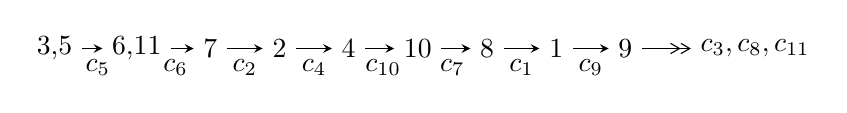
\begin{tikzpicture}[x=25pt, y=7pt]
	% node
	\node (A0) at (-1/8, 0) {3,5};
	\node (A1) at (17/16, 0) {6,11};
	\node (A2) at (17/8, 0) {7};
	\node (A3) at (25/8, 0) {2};
	\node (A4) at (33/8, 0) {4};
	\node (A5) at (41/8, 0) {10};
	\node (A6) at (49/8, 0) {8};
	\node (A7) at (57/8, 0) {1};
	\node (A8) at (65/8, 0) {9};
	\node (C1) at (1/2, -1) {$c_{5}$};
	\node (C2) at (13/8, -1) {$c_{6}$};
	\node (C3) at (21/8, -1) {$c_{2}$};
	\node (C4) at (29/8, -1) {$c_{4}$};
	\node (C5) at (37/8, -1) {$c_{10}$};
	\node (C6) at (45/8, -1) {$c_{7}$};
	\node (C7) at (53/8, -1) {$c_{1}$};
	\node (C8) at (61/8, -1) {$c_{9}$};
	\node (A9) at (10, 0) {$c_{3},c_{8},c_{11}$};

	% edge
	\draw[->,>=stealth]	
	(A0) edge (A1) (A1) edge (A2) (A2) edge (A3) (A3) edge (A4) (A4) edge (A5) (A5) edge (A6) (A6) edge (A7) (A7) edge (A8) ;
	\draw[->>,>={angle 60}]	
	(A8) edge (A9);
\end{tikzpicture} \\ 

\end{tabular} \\

\footnotetext{
The image of knot diagram is generated by the software ``\textbf{Draw programme}" developed by Andrew Bartholomew(\url{http://www.layer8.co.uk/maths/draw/index.htm\#Running-draw}), where we modified some parts for our purpose(\url{https://github.com/CATsTAILs/LinksPainter}).
}\phantom \\ \newline 
\centering \textbf{Ideals for irreducible components\footnotemark of $X_{\text{par}}$} 
 
\begin{align*}
I^u_{1}&=\langle 
1.44183\times10^{20} u^{19}-4.62808\times10^{20} u^{18}+\cdots+4.02960\times10^{22} b+1.32550\times10^{22},\\
\phantom{I^u_{1}}&\phantom{= \langle  }5.38510\times10^{21} u^{19}-1.93058\times10^{22} u^{18}+\cdots+5.64145\times10^{23} a-1.58764\times10^{23},\;u^{20}-3 u^{19}+\cdots+50 u+28\rangle \\
I^u_{2}&=\langle 
8.27426\times10^{22} a u^{24}+2.16729\times10^{23} u^{24}+\cdots-8.08063\times10^{23} a-2.16180\times10^{24},\\
\phantom{I^u_{2}}&\phantom{= \langle  }1.10607\times10^{23} a u^{24}-4.35547\times10^{23} u^{24}+\cdots-2.26434\times10^{24} a+5.35326\times10^{24},\;u^{25}+2 u^{24}+\cdots-18 u+5\rangle \\
I^u_{3}&=\langle 
-498 u^9 a+411 u^9+\cdots-538 a-71,\;33 u^9 a-50 u^9+\cdots+36 a+14,\\
\phantom{I^u_{3}}&\phantom{= \langle  }u^{10}+u^9+u^8- u^7-7 u^6-6 u^5-4 u^4- u^3+4 u^2-1\rangle \\
I^u_{4}&=\langle 
b+u,\;a- u+1,\;u^3+u+1\rangle \\
\\
\end{align*}
\raggedright * 4 irreducible components of $\dim_{\mathbb{C}}=0$, with total 93 representations.\\
\footnotetext{All coefficients of polynomials are rational numbers. But the coefficients are sometimes approximated in decimal forms when there is not enough margin.}
\newpage
\renewcommand{\arraystretch}{1}
\centering \section*{I. $I^u_{1}= \langle 1.44\times10^{20} u^{19}-4.63\times10^{20} u^{18}+\cdots+4.03\times10^{22} b+1.33\times10^{22},\;5.39\times10^{21} u^{19}-1.93\times10^{22} u^{18}+\cdots+5.64\times10^{23} a-1.59\times10^{23},\;u^{20}-3 u^{19}+\cdots+50 u+28 \rangle$}
\flushleft \textbf{(i) Arc colorings}\\
\begin{tabular}{m{7pt} m{180pt} m{7pt} m{180pt} }
\flushright $a_{3}=$&$\begin{pmatrix}0\\u\end{pmatrix}$ \\
\flushright $a_{5}=$&$\begin{pmatrix}1\\0\end{pmatrix}$ \\
\flushright $a_{6}=$&$\begin{pmatrix}1\\u^2\end{pmatrix}$ \\
\flushright $a_{11}=$&$\begin{pmatrix}-0.00954560 u^{19}+0.0342214 u^{18}+\cdots-2.04736 u+0.281424\\-0.00357808 u^{19}+0.0114852 u^{18}+\cdots-1.57985 u-0.328941\end{pmatrix}$ \\
\flushright $a_{7}=$&$\begin{pmatrix}0.00788039 u^{19}-0.0328040 u^{18}+\cdots-0.518617 u+0.751134\\0.00598606 u^{19}-0.0182745 u^{18}+\cdots+0.965413 u-0.0154483\end{pmatrix}$ \\
\flushright $a_{2}=$&$\begin{pmatrix}u\\u\end{pmatrix}$ \\
\flushright $a_{4}=$&$\begin{pmatrix}-0.0104192 u^{19}+0.0403606 u^{18}+\cdots-0.479468 u+0.453996\\0.00910287 u^{19}-0.0324780 u^{18}+\cdots+0.974959 u+0.291739\end{pmatrix}$ \\
\flushright $a_{10}=$&$\begin{pmatrix}-0.0131237 u^{19}+0.0457066 u^{18}+\cdots-3.62721 u-0.0475176\\-0.00357808 u^{19}+0.0114852 u^{18}+\cdots-1.57985 u-0.328941\end{pmatrix}$ \\
\flushright $a_{8}=$&$\begin{pmatrix}-0.0117479 u^{19}+0.0388218 u^{18}+\cdots-2.47010 u+0.992450\\-0.00558459 u^{19}+0.0212055 u^{18}+\cdots-0.758704 u-0.267277\end{pmatrix}$ \\
\flushright $a_{1}=$&$\begin{pmatrix}0.000551726 u^{19}+0.00433088 u^{18}+\cdots+2.81102 u+0.992999\\-0.00916278 u^{19}+0.0352104 u^{18}+\cdots+0.357114 u-0.220651\end{pmatrix}$ \\
\flushright $a_{9}=$&$\begin{pmatrix}-0.0117479 u^{19}+0.0388218 u^{18}+\cdots-2.47010 u+0.992450\\-0.00633555 u^{19}+0.0263534 u^{18}+\cdots-0.608667 u-0.367463\end{pmatrix}$\\ \flushright $a_{9}=$&$\begin{pmatrix}-0.0117479 u^{19}+0.0388218 u^{18}+\cdots-2.47010 u+0.992450\\-0.00633555 u^{19}+0.0263534 u^{18}+\cdots-0.608667 u-0.367463\end{pmatrix}$\\&\end{tabular}
\flushleft \textbf{(ii) Obstruction class $= -1$}\\~\\
\flushleft \textbf{(iii) Cusp Shapes $= -\frac{2008394464227286266247}{20148019962096448350151} u^{19}+\frac{6462622260672532812482}{20148019962096448350151} u^{18}+\cdots-\frac{48150419926932042591458}{20148019962096448350151} u-\frac{133443328465178993232190}{20148019962096448350151}$}\\~\\
\newpage\renewcommand{\arraystretch}{1}
\flushleft \textbf{(iv) u-Polynomials at the component}\newline \\
\begin{tabular}{m{50pt}|m{274pt}}
Crossings & \hspace{64pt}u-Polynomials at each crossing \\
\hline $$\begin{aligned}c_{1},c_{6}\end{aligned}$$&$\begin{aligned}
&u^{20}-5 u^{19}+\cdots+24 u-8
\end{aligned}$\\
\hline $$\begin{aligned}c_{2},c_{5}\end{aligned}$$&$\begin{aligned}
&u^{20}-3 u^{19}+\cdots+50 u+28
\end{aligned}$\\
\hline $$\begin{aligned}c_{3},c_{4}\end{aligned}$$&$\begin{aligned}
&u^{20}- u^{19}+\cdots-3 u^2+1
\end{aligned}$\\
\hline $$\begin{aligned}c_{7},c_{11}\end{aligned}$$&$\begin{aligned}
&u^{20}-2 u^{19}+\cdots-5 u-1
\end{aligned}$\\
\hline $$\begin{aligned}c_{8},c_{10}\end{aligned}$$&$\begin{aligned}
&u^{20}+9 u^{18}+\cdots+5 u-1
\end{aligned}$\\
\hline $$\begin{aligned}c_{9}\end{aligned}$$&$\begin{aligned}
&u^{20}+5 u^{19}+\cdots+192 u+32
\end{aligned}$\\
\hline
\end{tabular}\\~\\
\newpage\renewcommand{\arraystretch}{1}
\flushleft \textbf{(v) Riley Polynomials at the component}\newline \\
\begin{tabular}{m{50pt}|m{274pt}}
Crossings & \hspace{64pt}Riley Polynomials at each crossing \\
\hline $$\begin{aligned}c_{1},c_{6}\end{aligned}$$&$\begin{aligned}
&y^{20}+19 y^{19}+\cdots+384 y+64
\end{aligned}$\\
\hline $$\begin{aligned}c_{2},c_{5}\end{aligned}$$&$\begin{aligned}
&y^{20}+11 y^{19}+\cdots+6180 y+784
\end{aligned}$\\
\hline $$\begin{aligned}c_{3},c_{4}\end{aligned}$$&$\begin{aligned}
&y^{20}-3 y^{19}+\cdots-6 y+1
\end{aligned}$\\
\hline $$\begin{aligned}c_{7},c_{11}\end{aligned}$$&$\begin{aligned}
&y^{20}+24 y^{18}+\cdots-79 y+1
\end{aligned}$\\
\hline $$\begin{aligned}c_{8},c_{10}\end{aligned}$$&$\begin{aligned}
&y^{20}+18 y^{19}+\cdots+13 y+1
\end{aligned}$\\
\hline $$\begin{aligned}c_{9}\end{aligned}$$&$\begin{aligned}
&y^{20}+y^{19}+\cdots-14336 y+1024
\end{aligned}$\\
\hline
\end{tabular}\\~\\
\newpage\flushleft \textbf{(vi) Complex Volumes and Cusp Shapes}
$$\begin{array}{c|c|c}  
\text{Solutions to }I^u_{1}& \I (\text{vol} + \sqrt{-1}CS) & \text{Cusp shape}\\
 \hline 
\begin{aligned}
u &= \phantom{-}0.860797 + 0.516146 I \\
a &= -0.749789 - 0.590643 I \\
b &= -0.155130 - 0.305377 I\end{aligned}
 & -0.02958 - 4.97799 I & -5.29605 + 5.59335 I \\ \hline\begin{aligned}
u &= \phantom{-}0.860797 - 0.516146 I \\
a &= -0.749789 + 0.590643 I \\
b &= -0.155130 + 0.305377 I\end{aligned}
 & -0.02958 + 4.97799 I & -5.29605 - 5.59335 I \\ \hline\begin{aligned}
u &= -0.837495\phantom{ +0.000000I} \\
a &= \phantom{-}1.44067\phantom{ +0.000000I} \\
b &= -0.563826\phantom{ +0.000000I}\end{aligned}
 & -4.10423\phantom{ +0.000000I} & \phantom{-}8.28190\phantom{ +0.000000I} \\ \hline\begin{aligned}
u &= -0.127511 + 1.189810 I \\
a &= -0.55333 - 1.51288 I \\
b &= -0.265516 + 1.136880 I\end{aligned}
 & \phantom{-}5.89336 + 2.36950 I & \phantom{-}5.34088 - 5.91566 I \\ \hline\begin{aligned}
u &= -0.127511 - 1.189810 I \\
a &= -0.55333 + 1.51288 I \\
b &= -0.265516 - 1.136880 I\end{aligned}
 & \phantom{-}5.89336 - 2.36950 I & \phantom{-}5.34088 + 5.91566 I \\ \hline\begin{aligned}
u &= -1.206690 + 0.010929 I \\
a &= \phantom{-}0.309849 - 0.484836 I \\
b &= \phantom{-}0.275436 - 1.241550 I\end{aligned}
 & -1.50701 - 0.96018 I & -11.18870 + 6.49006 I \\ \hline\begin{aligned}
u &= -1.206690 - 0.010929 I \\
a &= \phantom{-}0.309849 + 0.484836 I \\
b &= \phantom{-}0.275436 + 1.241550 I\end{aligned}
 & -1.50701 + 0.96018 I & -11.18870 - 6.49006 I \\ \hline\begin{aligned}
u &= -0.044384 + 1.389540 I \\
a &= -0.092328 - 1.185210 I \\
b &= -0.230707 + 0.577747 I\end{aligned}
 & \phantom{-}3.02537 + 1.86293 I & -7.79633 - 3.80746 I \\ \hline\begin{aligned}
u &= -0.044384 - 1.389540 I \\
a &= -0.092328 + 1.185210 I \\
b &= -0.230707 - 0.577747 I\end{aligned}
 & \phantom{-}3.02537 - 1.86293 I & -7.79633 + 3.80746 I \\ \hline\begin{aligned}
u &= -0.495317\phantom{ +0.000000I} \\
a &= \phantom{-}0.784881\phantom{ +0.000000I} \\
b &= \phantom{-}0.562448\phantom{ +0.000000I}\end{aligned}
 & -0.861131\phantom{ +0.000000I} & -11.6540\phantom{ +0.000000I}\\
 \hline 
 \end{array}$$\newpage$$\begin{array}{c|c|c}  
\text{Solutions to }I^u_{1}& \I (\text{vol} + \sqrt{-1}CS) & \text{Cusp shape}\\
 \hline 
\begin{aligned}
u &= -0.008487 + 0.397854 I \\
a &= \phantom{-}0.665300 - 0.862267 I \\
b &= -0.433094 - 0.565353 I\end{aligned}
 & \phantom{-}1.66626 + 1.83421 I & -0.60394 - 1.52765 I \\ \hline\begin{aligned}
u &= -0.008487 - 0.397854 I \\
a &= \phantom{-}0.665300 + 0.862267 I \\
b &= -0.433094 + 0.565353 I\end{aligned}
 & \phantom{-}1.66626 - 1.83421 I & -0.60394 + 1.52765 I \\ \hline\begin{aligned}
u &= \phantom{-}1.70479 + 0.08565 I \\
a &= \phantom{-}0.138055 - 0.057007 I \\
b &= \phantom{-}0.519057 + 1.305600 I\end{aligned}
 & \phantom{-}2.91415 - 8.59875 I & -1.50122 + 6.80502 I \\ \hline\begin{aligned}
u &= \phantom{-}1.70479 - 0.08565 I \\
a &= \phantom{-}0.138055 + 0.057007 I \\
b &= \phantom{-}0.519057 - 1.305600 I\end{aligned}
 & \phantom{-}2.91415 + 8.59875 I & -1.50122 - 6.80502 I \\ \hline\begin{aligned}
u &= -0.47740 + 1.67811 I \\
a &= \phantom{-}0.103149 + 1.154610 I \\
b &= \phantom{-}1.18053 - 1.97776 I\end{aligned}
 & \phantom{-}4.37107 + 7.54282 I & -5.65623 - 11.11643 I \\ \hline\begin{aligned}
u &= -0.47740 - 1.67811 I \\
a &= \phantom{-}0.103149 - 1.154610 I \\
b &= \phantom{-}1.18053 + 1.97776 I\end{aligned}
 & \phantom{-}4.37107 - 7.54282 I & -5.65623 + 11.11643 I \\ \hline\begin{aligned}
u &= \phantom{-}0.68219 + 1.68930 I \\
a &= -0.198906 + 1.142030 I \\
b &= -1.17479 - 1.40102 I\end{aligned}
 & \phantom{-}8.5745 - 16.9983 I & -2.67254 + 8.37996 I \\ \hline\begin{aligned}
u &= \phantom{-}0.68219 - 1.68930 I \\
a &= -0.198906 - 1.142030 I \\
b &= -1.17479 + 1.40102 I\end{aligned}
 & \phantom{-}8.5745 + 16.9983 I & -2.67254 - 8.37996 I \\ \hline\begin{aligned}
u &= \phantom{-}0.78311 + 1.71850 I \\
a &= \phantom{-}0.300944 - 0.712043 I \\
b &= \phantom{-}0.284896 + 1.301190 I\end{aligned}
 & \phantom{-}8.00588 - 0.27607 I & \phantom{-}1.56028 - 0.31134 I \\ \hline\begin{aligned}
u &= \phantom{-}0.78311 - 1.71850 I \\
a &= \phantom{-}0.300944 + 0.712043 I \\
b &= \phantom{-}0.284896 - 1.301190 I\end{aligned}
 & \phantom{-}8.00588 + 0.27607 I & \phantom{-}1.56028 + 0.31134 I\\
 \hline 
 \end{array}$$\newpage\newpage\renewcommand{\arraystretch}{1}
\centering \section*{II. $I^u_{2}= \langle 8.27\times10^{22} a u^{24}+2.17\times10^{23} u^{24}+\cdots-8.08\times10^{23} a-2.16\times10^{24},\;1.11\times10^{23} a u^{24}-4.36\times10^{23} u^{24}+\cdots-2.26\times10^{24} a+5.35\times10^{24},\;u^{25}+2 u^{24}+\cdots-18 u+5 \rangle$}
\flushleft \textbf{(i) Arc colorings}\\
\begin{tabular}{m{7pt} m{180pt} m{7pt} m{180pt} }
\flushright $a_{3}=$&$\begin{pmatrix}0\\u\end{pmatrix}$ \\
\flushright $a_{5}=$&$\begin{pmatrix}1\\0\end{pmatrix}$ \\
\flushright $a_{6}=$&$\begin{pmatrix}1\\u^2\end{pmatrix}$ \\
\flushright $a_{11}=$&$\begin{pmatrix}a\\-0.715728 a u^{24}-1.87471 u^{24}+\cdots+6.98979 a+18.6997\end{pmatrix}$ \\
\flushright $a_{7}=$&$\begin{pmatrix}2.87565 a u^{24}-3.09074 u^{24}+\cdots-30.7439 a+31.3997\\0.805852 a u^{24}+1.72660 u^{24}+\cdots-8.29141 a-17.8506\end{pmatrix}$ \\
\flushright $a_{2}=$&$\begin{pmatrix}u\\u\end{pmatrix}$ \\
\flushright $a_{4}=$&$\begin{pmatrix}0.715728 a u^{24}+1.87471 u^{24}+\cdots-5.98979 a-18.6997\\-0.387518 a u^{24}-1.63688 u^{24}+\cdots+3.57864 a+19.9274\end{pmatrix}$ \\
\flushright $a_{10}=$&$\begin{pmatrix}-0.715728 a u^{24}-1.87471 u^{24}+\cdots+7.98979 a+18.6997\\-0.715728 a u^{24}-1.87471 u^{24}+\cdots+6.98979 a+18.6997\end{pmatrix}$ \\
\flushright $a_{8}=$&$\begin{pmatrix}-1.39796 a u^{24}-5.76946 u^{24}+\cdots+13.0810 a+58.4354\\0.379318 u^{24}+0.946149 u^{23}+\cdots-2.74341 u-5.54920\end{pmatrix}$ \\
\flushright $a_{1}=$&$\begin{pmatrix}-1.65828 a u^{24}+2.07471 u^{24}+\cdots+16.7481 a-22.2997\\-1.25756 a u^{24}+3.83734 u^{24}+\cdots+14.3782 a-42.0842\end{pmatrix}$ \\
\flushright $a_{9}=$&$\begin{pmatrix}-1.39796 a u^{24}-5.76946 u^{24}+\cdots+13.0810 a+58.4354\\-0.387518 a u^{24}-0.813602 u^{24}+\cdots+3.57864 a+7.89146\end{pmatrix}$\\ \flushright $a_{9}=$&$\begin{pmatrix}-1.39796 a u^{24}-5.76946 u^{24}+\cdots+13.0810 a+58.4354\\-0.387518 a u^{24}-0.813602 u^{24}+\cdots+3.57864 a+7.89146\end{pmatrix}$\\&\end{tabular}
\flushleft \textbf{(ii) Obstruction class $= -1$}\\~\\
\flushleft \textbf{(iii) Cusp Shapes $= -\frac{1156952596349356967504}{1993212416684380527497} u^{24}-\frac{3249366973641059899377}{1993212416684380527497} u^{23}+\cdots-\frac{66879505468638485855810}{1993212416684380527497} u+\frac{10075785679097148312488}{1993212416684380527497}$}\\~\\
\newpage\renewcommand{\arraystretch}{1}
\flushleft \textbf{(iv) u-Polynomials at the component}\newline \\
\begin{tabular}{m{50pt}|m{274pt}}
Crossings & \hspace{64pt}u-Polynomials at each crossing \\
\hline $$\begin{aligned}c_{1},c_{6}\end{aligned}$$&$\begin{aligned}
&u^{50}+5 u^{49}+\cdots+337800 u+93608
\end{aligned}$\\
\hline $$\begin{aligned}c_{2},c_{5}\end{aligned}$$&$\begin{aligned}
&(u^{25}+2 u^{24}+\cdots-18 u+5)^{2}
\end{aligned}$\\
\hline $$\begin{aligned}c_{3},c_{4}\end{aligned}$$&$\begin{aligned}
&u^{50}-4 u^{49}+\cdots+5 u-1
\end{aligned}$\\
\hline $$\begin{aligned}c_{7},c_{11}\end{aligned}$$&$\begin{aligned}
&u^{50}- u^{49}+\cdots+22 u-1
\end{aligned}$\\
\hline $$\begin{aligned}c_{8},c_{10}\end{aligned}$$&$\begin{aligned}
&u^{50}+3 u^{48}+\cdots-10342 u-3931
\end{aligned}$\\
\hline $$\begin{aligned}c_{9}\end{aligned}$$&$\begin{aligned}
&(u^{25}- u^{24}+\cdots-18 u+31)^{2}
\end{aligned}$\\
\hline
\end{tabular}\\~\\
\newpage\renewcommand{\arraystretch}{1}
\flushleft \textbf{(v) Riley Polynomials at the component}\newline \\
\begin{tabular}{m{50pt}|m{274pt}}
Crossings & \hspace{64pt}Riley Polynomials at each crossing \\
\hline $$\begin{aligned}c_{1},c_{6}\end{aligned}$$&$\begin{aligned}
&y^{50}+13 y^{49}+\cdots+42553508800 y+8762457664
\end{aligned}$\\
\hline $$\begin{aligned}c_{2},c_{5}\end{aligned}$$&$\begin{aligned}
&(y^{25}+24 y^{24}+\cdots-336 y-25)^{2}
\end{aligned}$\\
\hline $$\begin{aligned}c_{3},c_{4}\end{aligned}$$&$\begin{aligned}
&y^{50}+18 y^{48}+\cdots+143 y+1
\end{aligned}$\\
\hline $$\begin{aligned}c_{7},c_{11}\end{aligned}$$&$\begin{aligned}
&y^{50}-21 y^{49}+\cdots+244 y+1
\end{aligned}$\\
\hline $$\begin{aligned}c_{8},c_{10}\end{aligned}$$&$\begin{aligned}
&y^{50}+6 y^{49}+\cdots+33112428 y+15452761
\end{aligned}$\\
\hline $$\begin{aligned}c_{9}\end{aligned}$$&$\begin{aligned}
&(y^{25}-17 y^{24}+\cdots+12662 y-961)^{2}
\end{aligned}$\\
\hline
\end{tabular}\\~\\
\newpage\flushleft \textbf{(vi) Complex Volumes and Cusp Shapes}
$$\begin{array}{c|c|c}  
\text{Solutions to }I^u_{2}& \I (\text{vol} + \sqrt{-1}CS) & \text{Cusp shape}\\
 \hline 
\begin{aligned}
u &= -1.140650 + 0.267150 I \\
a &= \phantom{-}1.084710 + 0.611862 I \\
b &= \phantom{-}1.49229 + 0.92382 I\end{aligned}
 & -1.03856 + 1.14326 I & -10.5893 + 12.6521 I \\ \hline\begin{aligned}
u &= -1.140650 + 0.267150 I \\
a &= \phantom{-}0.113359 + 0.355439 I \\
b &= \phantom{-}0.633787 + 0.654814 I\end{aligned}
 & -1.03856 + 1.14326 I & -10.5893 + 12.6521 I \\ \hline\begin{aligned}
u &= -1.140650 - 0.267150 I \\
a &= \phantom{-}1.084710 - 0.611862 I \\
b &= \phantom{-}1.49229 - 0.92382 I\end{aligned}
 & -1.03856 - 1.14326 I & -10.5893 - 12.6521 I \\ \hline\begin{aligned}
u &= -1.140650 - 0.267150 I \\
a &= \phantom{-}0.113359 - 0.355439 I \\
b &= \phantom{-}0.633787 - 0.654814 I\end{aligned}
 & -1.03856 - 1.14326 I & -10.5893 - 12.6521 I \\ \hline\begin{aligned}
u &= -0.163146 + 1.252380 I \\
a &= -0.356875 - 0.754522 I \\
b &= -0.959590 + 0.451959 I\end{aligned}
 & \phantom{-}2.89680 + 2.76831 I & -5.67436 - 1.24863 I \\ \hline\begin{aligned}
u &= -0.163146 + 1.252380 I \\
a &= \phantom{-}0.223215 - 1.350440 I \\
b &= -0.670798 + 0.653559 I\end{aligned}
 & \phantom{-}2.89680 + 2.76831 I & -5.67436 - 1.24863 I \\ \hline\begin{aligned}
u &= -0.163146 - 1.252380 I \\
a &= -0.356875 + 0.754522 I \\
b &= -0.959590 - 0.451959 I\end{aligned}
 & \phantom{-}2.89680 - 2.76831 I & -5.67436 + 1.24863 I \\ \hline\begin{aligned}
u &= -0.163146 - 1.252380 I \\
a &= \phantom{-}0.223215 + 1.350440 I \\
b &= -0.670798 - 0.653559 I\end{aligned}
 & \phantom{-}2.89680 - 2.76831 I & -5.67436 + 1.24863 I \\ \hline\begin{aligned}
u &= \phantom{-}0.434385 + 1.315760 I \\
a &= -0.676723 + 0.897603 I \\
b &= -0.451415 - 0.840386 I\end{aligned}
 & \phantom{-}6.24414 - 3.55600 I & \phantom{-}4.03991 + 3.49531 I \\ \hline\begin{aligned}
u &= \phantom{-}0.434385 + 1.315760 I \\
a &= \phantom{-}0.14272 - 1.58350 I \\
b &= \phantom{-}1.25444 + 1.50173 I\end{aligned}
 & \phantom{-}6.24414 - 3.55600 I & \phantom{-}4.03991 + 3.49531 I\\
 \hline 
 \end{array}$$\newpage$$\begin{array}{c|c|c}  
\text{Solutions to }I^u_{2}& \I (\text{vol} + \sqrt{-1}CS) & \text{Cusp shape}\\
 \hline 
\begin{aligned}
u &= \phantom{-}0.434385 - 1.315760 I \\
a &= -0.676723 - 0.897603 I \\
b &= -0.451415 + 0.840386 I\end{aligned}
 & \phantom{-}6.24414 + 3.55600 I & \phantom{-}4.03991 - 3.49531 I \\ \hline\begin{aligned}
u &= \phantom{-}0.434385 - 1.315760 I \\
a &= \phantom{-}0.14272 + 1.58350 I \\
b &= \phantom{-}1.25444 - 1.50173 I\end{aligned}
 & \phantom{-}6.24414 + 3.55600 I & \phantom{-}4.03991 - 3.49531 I \\ \hline\begin{aligned}
u &= \phantom{-}0.15084 + 1.44113 I \\
a &= -0.365971 - 1.348100 I \\
b &= \phantom{-}1.12800 + 1.43516 I\end{aligned}
 & \phantom{-}6.70056 - 6.60168 I & \phantom{-}4.95046 + 12.30292 I \\ \hline\begin{aligned}
u &= \phantom{-}0.15084 + 1.44113 I \\
a &= \phantom{-}0.23756 + 1.60715 I \\
b &= -0.035729 - 0.763533 I\end{aligned}
 & \phantom{-}6.70056 - 6.60168 I & \phantom{-}4.95046 + 12.30292 I \\ \hline\begin{aligned}
u &= \phantom{-}0.15084 - 1.44113 I \\
a &= -0.365971 + 1.348100 I \\
b &= \phantom{-}1.12800 - 1.43516 I\end{aligned}
 & \phantom{-}6.70056 + 6.60168 I & \phantom{-}4.95046 - 12.30292 I \\ \hline\begin{aligned}
u &= \phantom{-}0.15084 - 1.44113 I \\
a &= \phantom{-}0.23756 - 1.60715 I \\
b &= -0.035729 + 0.763533 I\end{aligned}
 & \phantom{-}6.70056 + 6.60168 I & \phantom{-}4.95046 - 12.30292 I \\ \hline\begin{aligned}
u &= -0.148436 + 0.506372 I \\
a &= \phantom{-}0.388829 + 0.383713 I \\
b &= \phantom{-}1.118110 - 0.274856 I\end{aligned}
 & -2.53372 + 0.16719 I & -3.64574 - 0.21536 I \\ \hline\begin{aligned}
u &= -0.148436 + 0.506372 I \\
a &= \phantom{-}3.02455 + 0.27470 I \\
b &= -0.251824 - 0.797330 I\end{aligned}
 & -2.53372 + 0.16719 I & -3.64574 - 0.21536 I \\ \hline\begin{aligned}
u &= -0.148436 - 0.506372 I \\
a &= \phantom{-}0.388829 - 0.383713 I \\
b &= \phantom{-}1.118110 + 0.274856 I\end{aligned}
 & -2.53372 - 0.16719 I & -3.64574 + 0.21536 I \\ \hline\begin{aligned}
u &= -0.148436 - 0.506372 I \\
a &= \phantom{-}3.02455 - 0.27470 I \\
b &= -0.251824 + 0.797330 I\end{aligned}
 & -2.53372 - 0.16719 I & -3.64574 + 0.21536 I\\
 \hline 
 \end{array}$$\newpage$$\begin{array}{c|c|c}  
\text{Solutions to }I^u_{2}& \I (\text{vol} + \sqrt{-1}CS) & \text{Cusp shape}\\
 \hline 
\begin{aligned}
u &= \phantom{-}0.475339\phantom{ +0.000000I} \\
a &= \phantom{-}0.528924 + 0.781882 I \\
b &= -0.430675 + 0.809478 I\end{aligned}
 & \phantom{-}2.81112\phantom{ +0.000000I} & \phantom{-}0.202280\phantom{ +0.000000I} \\ \hline\begin{aligned}
u &= \phantom{-}0.475339\phantom{ +0.000000I} \\
a &= \phantom{-}0.528924 - 0.781882 I \\
b &= -0.430675 - 0.809478 I\end{aligned}
 & \phantom{-}2.81112\phantom{ +0.000000I} & \phantom{-}0.202280\phantom{ +0.000000I} \\ \hline\begin{aligned}
u &= -1.53222\phantom{ +0.000000I} \\
a &= \phantom{-}0.078790 + 0.191294 I \\
b &= \phantom{-}0.568791 - 1.033300 I\end{aligned}
 & \phantom{-}3.05217\phantom{ +0.000000I} & \phantom{-}0.159530\phantom{ +0.000000I} \\ \hline\begin{aligned}
u &= -1.53222\phantom{ +0.000000I} \\
a &= \phantom{-}0.078790 - 0.191294 I \\
b &= \phantom{-}0.568791 + 1.033300 I\end{aligned}
 & \phantom{-}3.05217\phantom{ +0.000000I} & \phantom{-}0.159530\phantom{ +0.000000I} \\ \hline\begin{aligned}
u &= \phantom{-}0.466383 + 0.024974 I \\
a &= \phantom{-}0.624833 - 0.860638 I \\
b &= -0.840463 - 0.646691 I\end{aligned}
 & \phantom{-}1.53850 - 4.51240 I & -4.65188 + 7.14304 I \\ \hline\begin{aligned}
u &= \phantom{-}0.466383 + 0.024974 I \\
a &= \phantom{-}1.42335 - 2.52636 I \\
b &= \phantom{-}0.735817 + 0.431578 I\end{aligned}
 & \phantom{-}1.53850 - 4.51240 I & -4.65188 + 7.14304 I \\ \hline\begin{aligned}
u &= \phantom{-}0.466383 - 0.024974 I \\
a &= \phantom{-}0.624833 + 0.860638 I \\
b &= -0.840463 + 0.646691 I\end{aligned}
 & \phantom{-}1.53850 + 4.51240 I & -4.65188 - 7.14304 I \\ \hline\begin{aligned}
u &= \phantom{-}0.466383 - 0.024974 I \\
a &= \phantom{-}1.42335 + 2.52636 I \\
b &= \phantom{-}0.735817 - 0.431578 I\end{aligned}
 & \phantom{-}1.53850 + 4.51240 I & -4.65188 - 7.14304 I \\ \hline\begin{aligned}
u &= \phantom{-}1.54406\phantom{ +0.000000I} \\
a &= -0.230436\phantom{ +0.000000I} \\
b &= \phantom{-}0.365605\phantom{ +0.000000I}\end{aligned}
 & -6.61075\phantom{ +0.000000I} & -51.2600\phantom{ +0.000000I} \\ \hline\begin{aligned}
u &= \phantom{-}1.54406\phantom{ +0.000000I} \\
a &= -1.77941\phantom{ +0.000000I} \\
b &= -1.23498\phantom{ +0.000000I}\end{aligned}
 & -6.61075\phantom{ +0.000000I} & -51.2600\phantom{ +0.000000I}\\
 \hline 
 \end{array}$$\newpage$$\begin{array}{c|c|c}  
\text{Solutions to }I^u_{2}& \I (\text{vol} + \sqrt{-1}CS) & \text{Cusp shape}\\
 \hline 
\begin{aligned}
u &= -0.18525 + 1.56503 I \\
a &= -0.482316 - 0.856149 I \\
b &= \phantom{-}0.583599 + 0.895127 I\end{aligned}
 & \phantom{-}3.52121 - 5.29385 I & -3.74916 + 8.30350 I \\ \hline\begin{aligned}
u &= -0.18525 + 1.56503 I \\
a &= \phantom{-}0.672798 - 0.276435 I \\
b &= \phantom{-}1.161330 + 0.309043 I\end{aligned}
 & \phantom{-}3.52121 - 5.29385 I & -3.74916 + 8.30350 I \\ \hline\begin{aligned}
u &= -0.18525 - 1.56503 I \\
a &= -0.482316 + 0.856149 I \\
b &= \phantom{-}0.583599 - 0.895127 I\end{aligned}
 & \phantom{-}3.52121 + 5.29385 I & -3.74916 - 8.30350 I \\ \hline\begin{aligned}
u &= -0.18525 - 1.56503 I \\
a &= \phantom{-}0.672798 + 0.276435 I \\
b &= \phantom{-}1.161330 - 0.309043 I\end{aligned}
 & \phantom{-}3.52121 + 5.29385 I & -3.74916 - 8.30350 I \\ \hline\begin{aligned}
u &= \phantom{-}0.003969 + 0.337154 I \\
a &= \phantom{-}0.650002 + 0.785649 I \\
b &= -1.171020 + 0.504584 I\end{aligned}
 & -0.56308 + 6.78110 I & \phantom{-}3.38343 - 3.19298 I \\ \hline\begin{aligned}
u &= \phantom{-}0.003969 + 0.337154 I \\
a &= \phantom{-}7.17919 - 1.72929 I \\
b &= -0.074163 + 0.750946 I\end{aligned}
 & -0.56308 + 6.78110 I & \phantom{-}3.38343 - 3.19298 I \\ \hline\begin{aligned}
u &= \phantom{-}0.003969 - 0.337154 I \\
a &= \phantom{-}0.650002 - 0.785649 I \\
b &= -1.171020 - 0.504584 I\end{aligned}
 & -0.56308 - 6.78110 I & \phantom{-}3.38343 + 3.19298 I \\ \hline\begin{aligned}
u &= \phantom{-}0.003969 - 0.337154 I \\
a &= \phantom{-}7.17919 + 1.72929 I \\
b &= -0.074163 - 0.750946 I\end{aligned}
 & -0.56308 - 6.78110 I & \phantom{-}3.38343 + 3.19298 I \\ \hline\begin{aligned}
u &= \phantom{-}0.19448 + 1.65842 I \\
a &= \phantom{-}0.422264 - 0.836955 I \\
b &= -1.43214 + 1.44496 I\end{aligned}
 & \phantom{-}7.41514 + 1.27639 I & \phantom{-}2.55128 - 0.67478 I \\ \hline\begin{aligned}
u &= \phantom{-}0.19448 + 1.65842 I \\
a &= -0.325781 + 0.877177 I \\
b &= -0.010779 - 1.084000 I\end{aligned}
 & \phantom{-}7.41514 + 1.27639 I & \phantom{-}2.55128 - 0.67478 I\\
 \hline 
 \end{array}$$\newpage$$\begin{array}{c|c|c}  
\text{Solutions to }I^u_{2}& \I (\text{vol} + \sqrt{-1}CS) & \text{Cusp shape}\\
 \hline 
\begin{aligned}
u &= \phantom{-}0.19448 - 1.65842 I \\
a &= \phantom{-}0.422264 + 0.836955 I \\
b &= -1.43214 - 1.44496 I\end{aligned}
 & \phantom{-}7.41514 - 1.27639 I & \phantom{-}2.55128 + 0.67478 I \\ \hline\begin{aligned}
u &= \phantom{-}0.19448 - 1.65842 I \\
a &= -0.325781 - 0.877177 I \\
b &= -0.010779 + 1.084000 I\end{aligned}
 & \phantom{-}7.41514 - 1.27639 I & \phantom{-}2.55128 + 0.67478 I \\ \hline\begin{aligned}
u &= -0.08719 + 1.73481 I \\
a &= \phantom{-}0.436377 + 0.874340 I \\
b &= -1.81263 - 1.76872 I\end{aligned}
 & \phantom{-}7.66608 + 6.24371 I & \phantom{-}4.09267 - 6.21663 I \\ \hline\begin{aligned}
u &= -0.08719 + 1.73481 I \\
a &= -0.211132 + 1.015010 I \\
b &= \phantom{-}0.62955 - 1.66105 I\end{aligned}
 & \phantom{-}7.66608 + 6.24371 I & \phantom{-}4.09267 - 6.21663 I \\ \hline\begin{aligned}
u &= -0.08719 - 1.73481 I \\
a &= \phantom{-}0.436377 - 0.874340 I \\
b &= -1.81263 + 1.76872 I\end{aligned}
 & \phantom{-}7.66608 - 6.24371 I & \phantom{-}4.09267 + 6.21663 I \\ \hline\begin{aligned}
u &= -0.08719 - 1.73481 I \\
a &= -0.211132 - 1.015010 I \\
b &= \phantom{-}0.62955 + 1.66105 I\end{aligned}
 & \phantom{-}7.66608 - 6.24371 I & \phantom{-}4.09267 + 6.21663 I \\ \hline\begin{aligned}
u &= -0.76896 + 1.70316 I \\
a &= -0.267227 - 1.109740 I \\
b &= -1.14143 + 1.30331 I\end{aligned}
 & \phantom{-}8.00509 + 8.45240 I & \phantom{-0.000000 } 0. - 6.49999 I \\ \hline\begin{aligned}
u &= -0.76896 + 1.70316 I \\
a &= \phantom{-}0.259474 + 0.720363 I \\
b &= \phantom{-}0.411624 - 1.049270 I\end{aligned}
 & \phantom{-}8.00509 + 8.45240 I & \phantom{-0.000000 } 0. - 6.49999 I \\ \hline\begin{aligned}
u &= -0.76896 - 1.70316 I \\
a &= -0.267227 + 1.109740 I \\
b &= -1.14143 - 1.30331 I\end{aligned}
 & \phantom{-}8.00509 - 8.45240 I & \phantom{-0.000000 -}0. + 6.49999 I \\ \hline\begin{aligned}
u &= -0.76896 - 1.70316 I \\
a &= \phantom{-}0.259474 - 0.720363 I \\
b &= \phantom{-}0.411624 + 1.049270 I\end{aligned}
 & \phantom{-}8.00509 - 8.45240 I & \phantom{-0.000000 -}0. + 6.49999 I\\
 \hline 
 \end{array}$$\newpage\newpage\renewcommand{\arraystretch}{1}
\centering \section*{III. $I^u_{3}= \langle -498 u^9 a+411 u^9+\cdots-538 a-71,\;33 u^9 a-50 u^9+\cdots+36 a+14,\;u^{10}+u^9+\cdots+4 u^2-1 \rangle$}
\flushleft \textbf{(i) Arc colorings}\\
\begin{tabular}{m{7pt} m{180pt} m{7pt} m{180pt} }
\flushright $a_{3}=$&$\begin{pmatrix}0\\u\end{pmatrix}$ \\
\flushright $a_{5}=$&$\begin{pmatrix}1\\0\end{pmatrix}$ \\
\flushright $a_{6}=$&$\begin{pmatrix}1\\u^2\end{pmatrix}$ \\
\flushright $a_{11}=$&$\begin{pmatrix}a\\0.256305 a u^{9}-0.211529 u^{9}+\cdots+0.276891 a+0.0365414\end{pmatrix}$ \\
\flushright $a_{7}=$&$\begin{pmatrix}-0.202265 a u^{9}+0.388574 u^{9}+\cdots+1.23932 a+1.61657\\-0.128667 a u^{9}-0.533196 u^{9}+\cdots-0.0386001 a+0.440041\end{pmatrix}$ \\
\flushright $a_{2}=$&$\begin{pmatrix}u\\u\end{pmatrix}$ \\
\flushright $a_{4}=$&$\begin{pmatrix}0.256305 a u^{9}-0.211529 u^{9}+\cdots-0.723109 a+0.0365414\\0.145651 a u^{9}+1.11889 u^{9}+\cdots-0.256305 a+0.935666\end{pmatrix}$ \\
\flushright $a_{10}=$&$\begin{pmatrix}0.256305 a u^{9}-0.211529 u^{9}+\cdots+1.27689 a+0.0365414\\0.256305 a u^{9}-0.211529 u^{9}+\cdots+0.276891 a+0.0365414\end{pmatrix}$ \\
\flushright $a_{8}=$&$\begin{pmatrix}-0.276891 a u^{9}+0.446217 u^{9}+\cdots-0.283067 a-0.566135\\-0.793103 u^{9}-1.10345 u^{8}+\cdots-1.24138 u-1.13793\end{pmatrix}$ \\
\flushright $a_{1}=$&$\begin{pmatrix}0.0386001 a u^{9}+0.594442 u^{9}+\cdots+0.511580 a-0.321668\\-0.325785 a u^{9}-0.513639 u^{9}+\cdots+0.202265 a-0.354092\end{pmatrix}$ \\
\flushright $a_{9}=$&$\begin{pmatrix}-0.276891 a u^{9}+0.446217 u^{9}+\cdots-0.283067 a-0.566135\\0.145651 a u^{9}-0.501801 u^{9}+\cdots-0.256305 a-1.65054\end{pmatrix}$\\ \flushright $a_{9}=$&$\begin{pmatrix}-0.276891 a u^{9}+0.446217 u^{9}+\cdots-0.283067 a-0.566135\\0.145651 a u^{9}-0.501801 u^{9}+\cdots-0.256305 a-1.65054\end{pmatrix}$\\&\end{tabular}
\flushleft \textbf{(ii) Obstruction class $= 1$}\\~\\
\flushleft \textbf{(iii) Cusp Shapes $= -\frac{70}{29} u^9-\frac{139}{29} u^8-\frac{166}{29} u^7+2 u^6+\frac{490}{29} u^5+\frac{1077}{29} u^4+\frac{738}{29} u^3+\frac{413}{29} u^2-\frac{44}{29} u-\frac{485}{29}$}\\~\\
\newpage\renewcommand{\arraystretch}{1}
\flushleft \textbf{(iv) u-Polynomials at the component}\newline \\
\begin{tabular}{m{50pt}|m{274pt}}
Crossings & \hspace{64pt}u-Polynomials at each crossing \\
\hline $$\begin{aligned}c_{1}\end{aligned}$$&$\begin{aligned}
&u^{20}-4 u^{19}+\cdots+24 u+8
\end{aligned}$\\
\hline $$\begin{aligned}c_{2}\end{aligned}$$&$\begin{aligned}
&(u^{10}- u^9+u^8+u^7-7 u^6+6 u^5-4 u^4+u^3+4 u^2-1)^2
\end{aligned}$\\
\hline $$\begin{aligned}c_{3}\end{aligned}$$&$\begin{aligned}
&u^{20}+7 u^{19}+\cdots- u-1
\end{aligned}$\\
\hline $$\begin{aligned}c_{4}\end{aligned}$$&$\begin{aligned}
&u^{20}-7 u^{19}+\cdots+u-1
\end{aligned}$\\
\hline $$\begin{aligned}c_{5}\end{aligned}$$&$\begin{aligned}
&(u^{10}+u^9+u^8- u^7-7 u^6-6 u^5-4 u^4- u^3+4 u^2-1)^2
\end{aligned}$\\
\hline $$\begin{aligned}c_{6}\end{aligned}$$&$\begin{aligned}
&u^{20}+4 u^{19}+\cdots-24 u+8
\end{aligned}$\\
\hline $$\begin{aligned}c_{7}\end{aligned}$$&$\begin{aligned}
&u^{20}+6 u^{19}+\cdots+8 u+1
\end{aligned}$\\
\hline $$\begin{aligned}c_{8}\end{aligned}$$&$\begin{aligned}
&u^{20}+u^{19}+\cdots-4 u-1
\end{aligned}$\\
\hline $$\begin{aligned}c_{9}\end{aligned}$$&$\begin{aligned}
&u^{20}-4 u^{18}+\cdots+146 u^2-31
\end{aligned}$\\
\hline $$\begin{aligned}c_{10}\end{aligned}$$&$\begin{aligned}
&u^{20}- u^{19}+\cdots+4 u-1
\end{aligned}$\\
\hline $$\begin{aligned}c_{11}\end{aligned}$$&$\begin{aligned}
&u^{20}-6 u^{19}+\cdots-8 u+1
\end{aligned}$\\
\hline
\end{tabular}\\~\\
\newpage\renewcommand{\arraystretch}{1}
\flushleft \textbf{(v) Riley Polynomials at the component}\newline \\
\begin{tabular}{m{50pt}|m{274pt}}
Crossings & \hspace{64pt}Riley Polynomials at each crossing \\
\hline $$\begin{aligned}c_{1},c_{6}\end{aligned}$$&$\begin{aligned}
&y^{20}-10 y^{19}+\cdots+832 y+64
\end{aligned}$\\
\hline $$\begin{aligned}c_{2},c_{5}\end{aligned}$$&$\begin{aligned}
&(y^{10}+y^9-11 y^8-11 y^7+39 y^6+24 y^5-54 y^4-19 y^3+24 y^2-8 y+1)^{2}
\end{aligned}$\\
\hline $$\begin{aligned}c_{3},c_{4}\end{aligned}$$&$\begin{aligned}
&y^{20}-9 y^{19}+\cdots+7 y+1
\end{aligned}$\\
\hline $$\begin{aligned}c_{7},c_{11}\end{aligned}$$&$\begin{aligned}
&y^{20}-2 y^{19}+\cdots-14 y+1
\end{aligned}$\\
\hline $$\begin{aligned}c_{8},c_{10}\end{aligned}$$&$\begin{aligned}
&y^{20}- y^{19}+\cdots-22 y+1
\end{aligned}$\\
\hline $$\begin{aligned}c_{9}\end{aligned}$$&$\begin{aligned}
&(y^{10}-4 y^9+\cdots+146 y-31)^{2}
\end{aligned}$\\
\hline
\end{tabular}\\~\\
\newpage\flushleft \textbf{(vi) Complex Volumes and Cusp Shapes}
$$\begin{array}{c|c|c}  
\text{Solutions to }I^u_{3}& \I (\text{vol} + \sqrt{-1}CS) & \text{Cusp shape}\\
 \hline 
\begin{aligned}
u &= -0.162027 + 1.093500 I \\
a &= -0.593689 + 0.666269 I \\
b &= -0.965025 - 0.562961 I\end{aligned}
 & \phantom{-}3.13638 - 3.94572 I & -1.58269 + 5.47828 I \\ \hline\begin{aligned}
u &= -0.162027 + 1.093500 I \\
a &= \phantom{-}0.91912 + 1.26340 I \\
b &= -0.554998 - 0.469577 I\end{aligned}
 & \phantom{-}3.13638 - 3.94572 I & -1.58269 + 5.47828 I \\ \hline\begin{aligned}
u &= -0.162027 - 1.093500 I \\
a &= -0.593689 - 0.666269 I \\
b &= -0.965025 + 0.562961 I\end{aligned}
 & \phantom{-}3.13638 + 3.94572 I & -1.58269 - 5.47828 I \\ \hline\begin{aligned}
u &= -0.162027 - 1.093500 I \\
a &= \phantom{-}0.91912 - 1.26340 I \\
b &= -0.554998 + 0.469577 I\end{aligned}
 & \phantom{-}3.13638 + 3.94572 I & -1.58269 - 5.47828 I \\ \hline\begin{aligned}
u &= -1.184430 + 0.161063 I \\
a &= -1.044950 - 0.712567 I \\
b &= -1.47068 - 1.35942 I\end{aligned}
 & -0.91356 + 1.34180 I & \phantom{-}8.0489 - 15.8298 I \\ \hline\begin{aligned}
u &= -1.184430 + 0.161063 I \\
a &= \phantom{-}0.266174 + 0.351567 I \\
b &= \phantom{-}0.614102 + 0.689658 I\end{aligned}
 & -0.91356 + 1.34180 I & \phantom{-}8.0489 - 15.8298 I \\ \hline\begin{aligned}
u &= -1.184430 - 0.161063 I \\
a &= -1.044950 + 0.712567 I \\
b &= -1.47068 + 1.35942 I\end{aligned}
 & -0.91356 - 1.34180 I & \phantom{-}8.0489 + 15.8298 I \\ \hline\begin{aligned}
u &= -1.184430 - 0.161063 I \\
a &= \phantom{-}0.266174 - 0.351567 I \\
b &= \phantom{-}0.614102 - 0.689658 I\end{aligned}
 & -0.91356 - 1.34180 I & \phantom{-}8.0489 + 15.8298 I \\ \hline\begin{aligned}
u &= \phantom{-}0.493258 + 0.211168 I \\
a &= \phantom{-}0.030687 + 0.614200 I \\
b &= -1.053900 - 0.481170 I\end{aligned}
 & -0.98335 - 6.94564 I & -13.6667 + 10.0962 I \\ \hline\begin{aligned}
u &= \phantom{-}0.493258 + 0.211168 I \\
a &= \phantom{-}1.07089 + 4.10487 I \\
b &= \phantom{-}0.278877 + 0.531389 I\end{aligned}
 & -0.98335 - 6.94564 I & -13.6667 + 10.0962 I\\
 \hline 
 \end{array}$$\newpage$$\begin{array}{c|c|c}  
\text{Solutions to }I^u_{3}& \I (\text{vol} + \sqrt{-1}CS) & \text{Cusp shape}\\
 \hline 
\begin{aligned}
u &= \phantom{-}0.493258 - 0.211168 I \\
a &= \phantom{-}0.030687 - 0.614200 I \\
b &= -1.053900 + 0.481170 I\end{aligned}
 & -0.98335 + 6.94564 I & -13.6667 - 10.0962 I \\ \hline\begin{aligned}
u &= \phantom{-}0.493258 - 0.211168 I \\
a &= \phantom{-}1.07089 - 4.10487 I \\
b &= \phantom{-}0.278877 - 0.531389 I\end{aligned}
 & -0.98335 + 6.94564 I & -13.6667 - 10.0962 I \\ \hline\begin{aligned}
u &= -0.510374\phantom{ +0.000000I} \\
a &= -0.34052 + 1.84999 I \\
b &= \phantom{-}0.789530 + 0.525018 I\end{aligned}
 & -3.56392\phantom{ +0.000000I} & -13.6180\phantom{ +0.000000I} \\ \hline\begin{aligned}
u &= -0.510374\phantom{ +0.000000I} \\
a &= -0.34052 - 1.84999 I \\
b &= \phantom{-}0.789530 - 0.525018 I\end{aligned}
 & -3.56392\phantom{ +0.000000I} & -13.6180\phantom{ +0.000000I} \\ \hline\begin{aligned}
u &= -0.19822 + 1.54173 I \\
a &= -0.059083 - 1.131320 I \\
b &= \phantom{-}0.371545 + 1.039520 I\end{aligned}
 & \phantom{-}6.26864 + 5.98904 I & -2.92384 - 3.18632 I \\ \hline\begin{aligned}
u &= -0.19822 + 1.54173 I \\
a &= -0.222760 + 1.238820 I \\
b &= \phantom{-}0.96108 - 1.49878 I\end{aligned}
 & \phantom{-}6.26864 + 5.98904 I & -2.92384 - 3.18632 I \\ \hline\begin{aligned}
u &= -0.19822 - 1.54173 I \\
a &= -0.059083 + 1.131320 I \\
b &= \phantom{-}0.371545 - 1.039520 I\end{aligned}
 & \phantom{-}6.26864 - 5.98904 I & -2.92384 + 3.18632 I \\ \hline\begin{aligned}
u &= -0.19822 - 1.54173 I \\
a &= -0.222760 - 1.238820 I \\
b &= \phantom{-}0.96108 + 1.49878 I\end{aligned}
 & \phantom{-}6.26864 - 5.98904 I & -2.92384 + 3.18632 I \\ \hline\begin{aligned}
u &= \phantom{-}1.61322\phantom{ +0.000000I} \\
a &= \phantom{-}1.68819\phantom{ +0.000000I} \\
b &= \phantom{-}1.26726\phantom{ +0.000000I}\end{aligned}
 & -6.51752\phantom{ +0.000000I} & \phantom{-}34.8670\phantom{ +0.000000I} \\ \hline\begin{aligned}
u &= \phantom{-}1.61322\phantom{ +0.000000I} \\
a &= \phantom{-}0.260087\phantom{ +0.000000I} \\
b &= -0.208312\phantom{ +0.000000I}\end{aligned}
 & -6.51752\phantom{ +0.000000I} & \phantom{-}34.8670\phantom{ +0.000000I}\\
 \hline 
 \end{array}$$\newpage\newpage\renewcommand{\arraystretch}{1}
\centering \section*{IV. $I^u_{4}= \langle b+u,\;a- u+1,\;u^3+u+1 \rangle$}
\flushleft \textbf{(i) Arc colorings}\\
\begin{tabular}{m{7pt} m{180pt} m{7pt} m{180pt} }
\flushright $a_{3}=$&$\begin{pmatrix}0\\u\end{pmatrix}$ \\
\flushright $a_{5}=$&$\begin{pmatrix}1\\0\end{pmatrix}$ \\
\flushright $a_{6}=$&$\begin{pmatrix}1\\u^2\end{pmatrix}$ \\
\flushright $a_{11}=$&$\begin{pmatrix}u-1\\- u\end{pmatrix}$ \\
\flushright $a_{7}=$&$\begin{pmatrix}- u^2-1\\u^2+1\end{pmatrix}$ \\
\flushright $a_{2}=$&$\begin{pmatrix}u\\u\end{pmatrix}$ \\
\flushright $a_{4}=$&$\begin{pmatrix}u^2- u+2\\- u^2+u-1\end{pmatrix}$ \\
\flushright $a_{10}=$&$\begin{pmatrix}-1\\- u\end{pmatrix}$ \\
\flushright $a_{8}=$&$\begin{pmatrix}-1\\u^2- u\end{pmatrix}$ \\
\flushright $a_{1}=$&$\begin{pmatrix}- u^2+u-1\\1\end{pmatrix}$ \\
\flushright $a_{9}=$&$\begin{pmatrix}-1\\- u\end{pmatrix}$\\ \flushright $a_{9}=$&$\begin{pmatrix}-1\\- u\end{pmatrix}$\\&\end{tabular}
\flushleft \textbf{(ii) Obstruction class $= 1$}\\~\\
\flushleft \textbf{(iii) Cusp Shapes $= -8 u^2+4 u-11$}\\~\\
\newpage\renewcommand{\arraystretch}{1}
\flushleft \textbf{(iv) u-Polynomials at the component}\newline \\
\begin{tabular}{m{50pt}|m{274pt}}
Crossings & \hspace{64pt}u-Polynomials at each crossing \\
\hline $$\begin{aligned}c_{1},c_{3}\end{aligned}$$&$\begin{aligned}
&u^3+u^2+1
\end{aligned}$\\
\hline $$\begin{aligned}c_{2},c_{8}\end{aligned}$$&$\begin{aligned}
&u^3+u-1
\end{aligned}$\\
\hline $$\begin{aligned}c_{4},c_{6}\end{aligned}$$&$\begin{aligned}
&u^3- u^2-1
\end{aligned}$\\
\hline $$\begin{aligned}c_{5},c_{10}\end{aligned}$$&$\begin{aligned}
&u^3+u+1
\end{aligned}$\\
\hline $$\begin{aligned}c_{7}\end{aligned}$$&$\begin{aligned}
&u^3+2 u^2+u-1
\end{aligned}$\\
\hline $$\begin{aligned}c_{9}\end{aligned}$$&$\begin{aligned}
&u^3
\end{aligned}$\\
\hline $$\begin{aligned}c_{11}\end{aligned}$$&$\begin{aligned}
&u^3-2 u^2+u+1
\end{aligned}$\\
\hline
\end{tabular}\\~\\
\newpage\renewcommand{\arraystretch}{1}
\flushleft \textbf{(v) Riley Polynomials at the component}\newline \\
\begin{tabular}{m{50pt}|m{274pt}}
Crossings & \hspace{64pt}Riley Polynomials at each crossing \\
\hline $$\begin{aligned}c_{1},c_{3},c_{4}\\c_{6}\end{aligned}$$&$\begin{aligned}
&y^3- y^2-2 y-1
\end{aligned}$\\
\hline $$\begin{aligned}c_{2},c_{5},c_{8}\\c_{10}\end{aligned}$$&$\begin{aligned}
&y^3+2 y^2+y-1
\end{aligned}$\\
\hline $$\begin{aligned}c_{7},c_{11}\end{aligned}$$&$\begin{aligned}
&y^3-2 y^2+5 y-1
\end{aligned}$\\
\hline $$\begin{aligned}c_{9}\end{aligned}$$&$\begin{aligned}
&y^3
\end{aligned}$\\
\hline
\end{tabular}\\~\\
\newpage\flushleft \textbf{(vi) Complex Volumes and Cusp Shapes}
$$\begin{array}{c|c|c}  
\text{Solutions to }I^u_{4}& \I (\text{vol} + \sqrt{-1}CS) & \text{Cusp shape}\\
 \hline 
\begin{aligned}
u &= \phantom{-}0.341164 + 1.161540 I \\
a &= -0.658836 + 1.161540 I \\
b &= -0.341164 - 1.161540 I\end{aligned}
 & \phantom{-}5.50124 - 1.58317 I & \phantom{-}0.22694 - 1.69425 I \\ \hline\begin{aligned}
u &= \phantom{-}0.341164 - 1.161540 I \\
a &= -0.658836 - 1.161540 I \\
b &= -0.341164 + 1.161540 I\end{aligned}
 & \phantom{-}5.50124 + 1.58317 I & \phantom{-}0.22694 + 1.69425 I \\ \hline\begin{aligned}
u &= -0.682328\phantom{ +0.000000I} \\
a &= -1.68233\phantom{ +0.000000I} \\
b &= \phantom{-}0.682328\phantom{ +0.000000I}\end{aligned}
 & -4.42273\phantom{ +0.000000I} & -17.4540\phantom{ +0.000000I}\\
 \hline 
 \end{array}$$\newpage
\newpage\renewcommand{\arraystretch}{1}
\centering \section*{ V. u-Polynomials}
\begin{tabular}{m{50pt}|m{274pt}}
Crossings & \hspace{64pt}u-Polynomials at each crossing \\
\hline $$\begin{aligned}c_{1}\end{aligned}$$&$\begin{aligned}
&(u^3+u^2+1)(u^{20}-5 u^{19}+\cdots+24 u-8)(u^{20}-4 u^{19}+\cdots+24 u+8)\\
&\cdot(u^{50}+5 u^{49}+\cdots+337800 u+93608)
\end{aligned}$\\
\hline $$\begin{aligned}c_{2}\end{aligned}$$&$\begin{aligned}
&(u^3+u-1)(u^{10}- u^9+u^8+u^7-7 u^6+6 u^5-4 u^4+u^3+4 u^2-1)^2\\
&\cdot(u^{20}-3 u^{19}+\cdots+50 u+28)(u^{25}+2 u^{24}+\cdots-18 u+5)^{2}
\end{aligned}$\\
\hline $$\begin{aligned}c_{3}\end{aligned}$$&$\begin{aligned}
&(u^3+u^2+1)(u^{20}- u^{19}+\cdots-3 u^2+1)(u^{20}+7 u^{19}+\cdots- u-1)\\
&\cdot(u^{50}-4 u^{49}+\cdots+5 u-1)
\end{aligned}$\\
\hline $$\begin{aligned}c_{4}\end{aligned}$$&$\begin{aligned}
&(u^3- u^2-1)(u^{20}-7 u^{19}+\cdots+u-1)(u^{20}- u^{19}+\cdots-3 u^2+1)\\
&\cdot(u^{50}-4 u^{49}+\cdots+5 u-1)
\end{aligned}$\\
\hline $$\begin{aligned}c_{5}\end{aligned}$$&$\begin{aligned}
&(u^3+u+1)(u^{10}+u^9+u^8- u^7-7 u^6-6 u^5-4 u^4- u^3+4 u^2-1)^2\\
&\cdot(u^{20}-3 u^{19}+\cdots+50 u+28)(u^{25}+2 u^{24}+\cdots-18 u+5)^{2}
\end{aligned}$\\
\hline $$\begin{aligned}c_{6}\end{aligned}$$&$\begin{aligned}
&(u^3- u^2-1)(u^{20}-5 u^{19}+\cdots+24 u-8)(u^{20}+4 u^{19}+\cdots-24 u+8)\\
&\cdot(u^{50}+5 u^{49}+\cdots+337800 u+93608)
\end{aligned}$\\
\hline $$\begin{aligned}c_{7}\end{aligned}$$&$\begin{aligned}
&(u^3+2 u^2+u-1)(u^{20}-2 u^{19}+\cdots-5 u-1)(u^{20}+6 u^{19}+\cdots+8 u+1)\\
&\cdot(u^{50}- u^{49}+\cdots+22 u-1)
\end{aligned}$\\
\hline $$\begin{aligned}c_{8}\end{aligned}$$&$\begin{aligned}
&(u^3+u-1)(u^{20}+9 u^{18}+\cdots+5 u-1)(u^{20}+u^{19}+\cdots-4 u-1)\\
&\cdot(u^{50}+3 u^{48}+\cdots-10342 u-3931)
\end{aligned}$\\
\hline $$\begin{aligned}c_{9}\end{aligned}$$&$\begin{aligned}
&u^3(u^{20}-4 u^{18}+\cdots+146 u^{2}-31)(u^{20}+5 u^{19}+\cdots+192 u+32)\\
&\cdot(u^{25}- u^{24}+\cdots-18 u+31)^{2}
\end{aligned}$\\
\hline $$\begin{aligned}c_{10}\end{aligned}$$&$\begin{aligned}
&(u^3+u+1)(u^{20}+9 u^{18}+\cdots+5 u-1)(u^{20}- u^{19}+\cdots+4 u-1)\\
&\cdot(u^{50}+3 u^{48}+\cdots-10342 u-3931)
\end{aligned}$\\
\hline $$\begin{aligned}c_{11}\end{aligned}$$&$\begin{aligned}
&(u^3-2 u^2+u+1)(u^{20}-6 u^{19}+\cdots-8 u+1)(u^{20}-2 u^{19}+\cdots-5 u-1)\\
&\cdot(u^{50}- u^{49}+\cdots+22 u-1)
\end{aligned}$\\
\hline
\end{tabular}\newpage\renewcommand{\arraystretch}{1}
\centering \section*{ VI. Riley Polynomials}
\begin{tabular}{m{50pt}|m{274pt}}
Crossings & \hspace{64pt}Riley Polynomials at each crossing \\
\hline $$\begin{aligned}c_{1},c_{6}\end{aligned}$$&$\begin{aligned}
&(y^3- y^2-2 y-1)(y^{20}-10 y^{19}+\cdots+832 y+64)\\
&\cdot(y^{20}+19 y^{19}+\cdots+384 y+64)\\
&\cdot(y^{50}+13 y^{49}+\cdots+42553508800 y+8762457664)
\end{aligned}$\\
\hline $$\begin{aligned}c_{2},c_{5}\end{aligned}$$&$\begin{aligned}
&(y^3+2 y^2+y-1)\\
&\cdot(y^{10}+y^9-11 y^8-11 y^7+39 y^6+24 y^5-54 y^4-19 y^3+24 y^2-8 y+1)^{2}\\
&\cdot(y^{20}+11 y^{19}+\cdots+6180 y+784)(y^{25}+24 y^{24}+\cdots-336 y-25)^{2}
\end{aligned}$\\
\hline $$\begin{aligned}c_{3},c_{4}\end{aligned}$$&$\begin{aligned}
&(y^3- y^2-2 y-1)(y^{20}-9 y^{19}+\cdots+7 y+1)(y^{20}-3 y^{19}+\cdots-6 y+1)\\
&\cdot(y^{50}+18 y^{48}+\cdots+143 y+1)
\end{aligned}$\\
\hline $$\begin{aligned}c_{7},c_{11}\end{aligned}$$&$\begin{aligned}
&(y^3-2 y^2+5 y-1)(y^{20}+24 y^{18}+\cdots-79 y+1)\\
&\cdot(y^{20}-2 y^{19}+\cdots-14 y+1)(y^{50}-21 y^{49}+\cdots+244 y+1)
\end{aligned}$\\
\hline $$\begin{aligned}c_{8},c_{10}\end{aligned}$$&$\begin{aligned}
&(y^3+2 y^2+y-1)(y^{20}- y^{19}+\cdots-22 y+1)\\
&\cdot(y^{20}+18 y^{19}+\cdots+13 y+1)\\
&\cdot(y^{50}+6 y^{49}+\cdots+33112428 y+15452761)
\end{aligned}$\\
\hline $$\begin{aligned}c_{9}\end{aligned}$$&$\begin{aligned}
&y^3(y^{10}-4 y^9+\cdots+146 y-31)^{2}(y^{20}+y^{19}+\cdots-14336 y+1024)\\
&\cdot(y^{25}-17 y^{24}+\cdots+12662 y-961)^{2}
\end{aligned}$\\
\hline
\end{tabular}
\vskip 2pc
\end{document}